\documentclass[twocolumn,prd,floatfix,preprintnumbers,a4paper,nofootinbib,superscriptaddress]{revtex4-1}

\usepackage{epsfig}
\usepackage{graphics}
\usepackage{graphicx}
\usepackage{amsmath,amssymb,mathtools}
\usepackage{amsfonts}
\usepackage{bm,soul}
\usepackage[usenames,dvipsnames]{color}
\usepackage{amssymb}
\usepackage{url}
\usepackage{psfrag}
\usepackage{times}
\usepackage[varg]{txfonts}
\usepackage[colorlinks, pdfborder={0 0 0}]{hyperref}
\usepackage{lineno}
\usepackage{verbatim}
\definecolor{LinkColor}{rgb}{0.75, 0, 0}
\definecolor{CiteColor}{rgb}{0.75, 0, 0}
\definecolor{UrlColor}{rgb}{0, 0, 0.75}
\hypersetup{linkcolor=LinkColor}
\hypersetup{citecolor=CiteColor}
\hypersetup{urlcolor=UrlColor}
\usepackage[utf8]{inputenc}
\usepackage{ulem}
\normalem
\hoffset -0.17in
\voffset 0.3in
\textheight 10in

%%%%%%%%%%%%%%%%%%%%%%%%%%%%%%%% Useful Definitions %%%%%%%%%%%%%%%%%%%%%%%%%%%%%%%%%%%%%%%%%

% definitions


\usepackage{inputenc}
\usepackage{pgfplots}
\usepackage{tikz}
\usetikzlibrary{shapes,arrows}
\usetikzlibrary{positioning}
\usetikzlibrary{backgrounds}

\def\singleline{
	\begin{center}
	\line(1,0){250}
	\end{center}
}

\newenvironment{aside}
    {\begin{addmargin}[1em]{2em}% 2em left, 1em right
\begin{center} \noindent\rule{0.65\paperwidth}{0.4pt} \end{center}
    }
    {
    \begin{center} \noindent\rule{0.65\paperwidth}{0.4pt} \end{center}
\end{addmargin}
    }

% CUSTOM COMMANDS
\newcommand\xquote[1]{``#1"}
\newcommand\psinr[2]{$\psi_{{#1}{#2}}^{NR}$}
% \newcommand\red[1]{{\color{red} #1}}
\newcommand\red[1]{{\color[rgb]{0.75,0.0,0.0} #1}}
\newcommand\green[1]{{\color[rgb]{0.0,0.60,0.08} #1}}
\newcommand\blue[1]{{\color[rgb]{0,0.20,0.65} #1}}
\newcommand\bluey[1]{{\color[rgb]{0.11,0.20,0.4} #1}}
\newcommand\gray[1]{{\color[rgb]{0.7,0.70,0.7} #1}}
\newcommand\grey[1]{{\color[rgb]{0.7,0.70,0.7} #1}}
\newcommand\white[1]{{\color[rgb]{1,1,1} #1}}
\newcommand\darkgray[1]{{\color[rgb]{0.3,0.30,0.3} #1}}
\newcommand\orange[1]{{\color[rgb]{.86,0.24,0.08} #1}}
\newcommand\purple[1]{{\color[rgb]{0.45,0.10,0.45} #1}}
\newcommand\note[1]{\colorbox[rgb]{0.85,0.94,1}{\textcolor{black}{\textsc{\textsf{#1}}}}}

%
\newcommand*{\figfactor}{0.495}

% Math symbols
% ###################################### %
%\def\mh{{\hat{h}}} % model  for strain
\def\m#1{{\hat{#1}}} % model  for strain
\def\ma#1{{\hat{#1}_{\bm{a}}}} % model  for strain
\newcommand{\var}[1]{\mathcal{{#1}}}
\newcommand{\mlam}{{\bm{\lambda}}}
\newcommand{\lam}{{\lambda}}
\newcommand{\mLam}{{\bm{\Lambda}}}
\newcommand{\bigo}[1]{{\cal O}({#1})}
\newcommand{\braket}[2]{ {\langle {#1} | {#2} \rangle} }
% ###################################### %

% ###################################### %
\definecolor{lightblue}{rgb}{.82,.88,0.95}
\definecolor{lightred}{rgb}{0.95,.86,0.86}
\definecolor{yellow}{rgb}{0.95,0.95,0.86}
\definecolor{green}{rgb}{.90,1,0.95}
\definecolor{lightpurple}{rgb}{.95,0.85,0.95}
% ###################################### %

\tikzset{
    vertex/.style = {
        circle,
        fill            = black,
        outer sep = 2pt,
        inner sep = 1pt,
    }
}


% CUSTOM DEFINITIONS
% ***************************************** %
\def\prd{Phys.Rev.D}
% ***************************************** %
\def\gt{Georgia Tech}
% ***************************************** %
\def\tk{Teukolsky}
% ***************************************** %
\def\mp{multipole}
% ***************************************** %
\def\ee{Einstein's equations}
% ***************************************** %
\def\toolkit#1{NRDA--Toolkit{#1}}
% \def\toolkit#1{Data Analysis Toolkit{#1}}
% ***************************************** %
\def\wf#1{waveform#1}
% ***************************************** %
\def\grad#1{gravitational radiation#1}
% ***************************************** %
\def\gr#1{General Relativity#1}
% ***************************************** %
\def\gwa#1{Gravitational Wave Astrophysics#1}
% ***************************************** %
\def\gwf#1{gravitational waveform#1}
% ***************************************** %
\def\psilm#1{\psi_{lm}#1}
% ***************************************** %
\def\rm#1{\mathrm{#1}}
% ***************************************** %


% Referencing
% ***************************************** %
\def\prt#1{Part~(\ref{#1})}
% ***************************************** %
\def\ap#1{Appendix~(\ref{#1})}
% ***************************************** %
\def\ch#1{Chapter~(\ref{#1})}
% ***************************************** %
\def\cch#1{Chapter~\ref{#1}}
% ***************************************** %
\newcommand{\chs}[2]{Chapters~(\ref{#1}-\ref{#2})}
% ***************************************** %
\newcommand{\cchs}[2]{Chapters~\ref{#1}-\ref{#2}}
% ***************************************** %
\def\sec#1{Section~(\ref{#1})}
% ***************************************** %
\def\csec#1{Section~\ref{#1}}
% ***************************************** %
\newcommand{\secs}[2]{Sections~(\ref{#1}-\ref{#2})}
% ***************************************** %
\def\fig#1{Figure~(\ref{#1})}
% \def\fig#1{\hyperref[#1]{Figure~\ref{#1}}}
% ***************************************** %
\def\cfig#1{Figure~\ref{#1}}
% ***************************************** %
\newcommand{\figs}[2]{Figures~(\ref{#1}-\ref{#2})}
% ***************************************** %
\def\eqn#1{Equation~(\ref{#1})}
% \def\eqn#1{\hyperref[#1]{Equation~\ref{#1}}} %
% ***************************************** %
\def\ceqn#1{Equation~\ref{#1}}
% ***************************************** %
\newcommand{\eqns}[2]{Equations~(\ref{#1}-\ref{#2})}
% ***************************************** %
\newcommand{\ceqns}[2]{Equations~\ref{#1}-\ref{#2}}
% ***************************************** %


% ***************************************** %
\def\da#1{data analysis#1}
% ***************************************** %
\def\lal#1{LIGO Analysis Library#1
  (LAL#1)\gdef\lal{LAL}}
% ***************************************** %
\def\nrda#1{\nr{} Data Analysis#1
  (NRDA#1)\gdef\nrda{NRDA}}
% ***************************************** %
\def\tt#1{\textit{transverse--traceless}#1
  (TT#1)\gdef\tt{TT}}
% ***************************************** %
\def\et#1{Einstein Telescope#1
  (ET#1)\gdef\et{ET}}
% ***************************************** %
\def\ego#1{European Gravitational Observatory#1
  (EGO#1)\gdef\ego{EGO}}
% ***************************************** %
\def\ligo#1{Laser Interferometer Gravitational Wave Observatory#1
  (LIGO#1)\gdef\ligo{LIGO}}
% ***************************************** %
\def\aligo#1{Advanced LIGO#1
  (Adv. LIGO#1)\gdef\aligo{Adv. LIGO}}
% ***************************************** %
\def\snr#1{signal to noise ratio#1
  (SNR#1)\gdef\snr{SNR}}
% ***************************************** %
\def\psd#1{power spectral density#1
  (PSD#1)\gdef\psd{PSD}}
% ***************************************** %
\def\rom#1{reduced order model#1
  (ROM#1)\gdef\rom{ROM}}
% ***************************************** %
\def\gatech#1{Georgia Tech#1}
% ***************************************** %


% ***************************************** %
%\def\bh#1{black hole#1
%  (BH#1)\gdef\bh{BH}}
\def\bh#1{black hole#1}
% ***************************************** %
%\def\bbh#1{binary black hole#1
%  (BBH#1)\gdef\bbh{BBH}}
\def\bbh#1{binary black hole#1}
% ***************************************** %
\def\bhb#1{\bh{} binary#1}
% ***************************************** %


% ***************************************** %
\def\qnm#1{Quasi-Normal Mode#1
  (QNM#1)\gdef\qnm{QNM}}
% ***************************************** %
\def\eob#1{Effective One Body#1
  (EOB#1)\gdef\eob{EOB}}
% ***************************************** %
\def\gw#1{gravitational wave#1}
%\def\gw#1{gravitational wave#1
%  (GW#1)\gdef\gw{GW}}
% ***************************************** %
\def\gwa#1{gravitational wave astronomy#1}
% ***************************************** %
\def\pn#1{Post-Newtonian#1}
%\def\pn#1{Post-Newtonian#1
%  (PN#1)\gdef\pn{PN}}
\def\pnl#1{post-Newtonian-like#1
  (PN-like#1)\gdef\pnl{PN-like}}
% ***************************************** %
\def\nr{Numerical Relativity}
\def\NR{{\text{NR}}}
%\def\nr{Numerical Relativity
%  (NR)\gdef\nr{NR}}
% ***************************************** %
\def\pt{\bh{} perturbation theory}
% ***************************************** %
\def\GOLS#1{\textit{greedy-OLS}#1}
% ***************************************** %
\def\rd{ringdown}
% ***************************************** %
\def\imr{inspiral, merger and \rd{}}
% ***************************************** %
\def\cbc#1{compact object coalescence#1}
% ***************************************** %
\def\bbc#1{binary black hole coalescence#1}
%\def\bbc#1{binary black hole coalescence#1
%  (BBC#1)\gdef\bbc{BBC}}
% ***************************************** %
\def\pc#1{principle component#1}
% ***************************************** %
\def\pca#1{principle component analysis#1
  (PCA#1)\gdef\pca{PCA}}
% ***************************************** %
\def\svd#1{Singular Value Decomposition#1
  (SVD#1)\gdef\svd{SVD}}
% ***************************************** %
\def\gs#1{Gram-Schmidt#1}
%\def\gs#1{Gram-Schmidt#1
%  (GS#1)\gdef\gs{GS}}
% ***************************************** %
% \newcommand{\DS}[1]{{\bf\color{red}{[DS: #1]}}}
% % ***************************************** %
% \newcommand{\LL}[1]{{\bf\blue{[LL: #1]}}}
% ***************************************** %
\newcommand*{\factor}{0.95} % for figure scale
\newcommand*{\rscale}{1.3}
% ***************************************** %

% ******************************************************* %
\def\study{work} % to be changed to "Letter" upon approval
% ******************************************************* %

\newcommand{\osum}{\operatornamewithlimits{
\hspace{-2pt}{\bigcup\hspace{-9.5pt}\circ}
}}

% commutative multiplication
\newcommand{\ox}{\operatornamewithlimits{
{\circ\hspace{-3.7pt}\cdot}
}}

% non-commutative multiplication
\newcommand{\cc}{ \circledcirc }

% general subtraction
\newcommand{\om}{ \mathrel{\raisebox{1pt}{$\scriptscriptstyle\circleddash$}} }






\newcommand{\hlgreen}[1]{\sethlcolor{green}\hl{#1}{\sethlcolor{yellow}}}
\newcommand{\hlyellow}[1]{\sethlcolor{yellow}\hl{#1}{\sethlcolor{yellow}}}
\newcommand{\hlblue}[1]{\sethlcolor{lightblue}\hl{#1}{\sethlcolor{yellow}}}
\newcommand{\hlred}[1]{\sethlcolor{lightred}\hl{#1}{\sethlcolor{yellow}}}
\newcommand{\hlpurple}[1]{\sethlcolor{lightpurple}\hl{#1}{\sethlcolor{yellow}}}

\newcommand{\hlbackground}[1]{\sethlcolor{green}\hl{#1}{\sethlcolor{yellow}}}
\newcommand{\hlproblem}[1]{\sethlcolor{yellow}\hl{#1}{\sethlcolor{yellow}}}
\newcommand{\hlmethods}[1]{\sethlcolor{lightblue}\hl{#1}{\sethlcolor{yellow}}}
\newcommand{\hlresults}[1]{\sethlcolor{lightred}\hl{#1}{\sethlcolor{yellow}}}
\newcommand{\hldiscussion}[1]{\sethlcolor{lightpurple}\hl{#1}{\sethlcolor{yellow}}}


% Richard's stuff

\newcommand\aap{\&A}
\newcommand\apss{APSS}
\newcommand\aaps{AAPS}
\newcommand\apjs{ApJ S}
\newcommand\aj{AJ}
\newcommand\apjl{ApJL}
\newcommand\mnras{MNRAS}
\newcommand\pasp{PASP}
\newcommand\araa{ARAA}
\newcommand\physrep{Phys. Rep.}

\newcommand\nrRequest{\textbf{NR INPUT?}}
\newcommand\richardBugFix{\textbf{\color{red}Richard will bugfix}}
\newcommand\editremark[1]{ {\color{red} #1}}
\newcommand\newtext[1]{{\bf #1}}
\newcommand\recentlychanged[1]{{\bf #1}}
\newcommand\hidetosubmit[1]{}
%
\newcommand\optional[1]{}
\newcommand\ForInternalReference[1]{}
\newcommand\embrace[1]{{[#1]}}
\newcommand\unit[1]{\, {\rm #1}}
\newcommand\mc{ {{\cal M}_c}}
\newcommand\Dho{ {D_{\rm H}^{(0)}}}
\newcommand\Dh{ {D_{\rm H}}}
\newcommand\Deff{{D_{\rm eff}}}  %
\newcommand\Dv{{D_{\rm v}}}      %
\newcommand\Dc{{D_c}}            %
\newcommand\Y[1]{Y^{(#1)}}


\newcommand\avL{\left< {\cal L}_{(a} {\cal L}_{b)} \right>}
\newcommand\WeylScalar{{\psi_4}}
\newcommand\WeylScalarFourier{{\tilde{\psi}_4{}}}
\newcommand\FourierWeylScalar{{\tilde{\psi}_4}}
\newcommand\WeylScalarCorot{R^{-1}{\psi_4}}

\newcommand\qmstate[1]{\left|#1\right>}
\newcommand\qmstateKet[1]{\left<#1\right|}
\newcommand\qmstateproduct[2]{\left<#1|#2\right>}
\newcommand\qmoperatorelement[3]{\left<#1\left|#2\right|#3\right>}
\newcommand\qmoperator[1]{{\bf #1}}
\newcommand\myvector[1]{{\mathbf{#1}}}
\newcommand\chip{{\boldsymbol{\chi}_+}}
\newcommand\chim{{\boldsymbol{\chi}_-}}

\newcommand\nSimulationsTotal{224}   %
\newcommand\nSimulationsNonprecessing{62}  %
\newcommand\ReferenceMassLow{100}      %
\newcommand\ReferenceMassMiddle{300}   %
\newcommand\ReferenceMassHigh{1000}   %


\newcommand\abbrvPSgrbs{PS-GRB}
\newcommand\abbrvCBC{CBC}

\newcommand{\cw}{\tilde{\omega}}
\newcommand{\CW}{\tilde{\Omega}}
\newcommand{\CWr}{{\Omega}^{\mathrm{r}}}
\newcommand{\CWc}{{\Omega}^{\mathrm{c}}}
\newcommand{\SC}{\mathcal{K}}
\newcommand{\CC}{\mathcal{C}}
\newcommand{\SCr}{\mathcal{K}^{\mathrm{r}}}
\newcommand{\SCc}{\mathcal{K}^{\mathrm{c}}}
\newcommand{\lalapprox}{\texttt{MMRDNS}}
\def\j{j_f}
\newcommand{\LL}{\bar{l}}
\newcommand{\MM}{\bar{m}}

\newcommand{\lmtitle}[2]{\vspace{-0.80cm} \begin{center} \noindent\rule{0.35\paperwidth}{0.3pt} \end{center} \vspace{-0.3cm}}

% \newcommand{\lmtitle}[2]{$(\LL,\MM) = ({#1},{#2}) $ \vspace{-0.5cm} \begin{center} \noindent\rule{0.35\paperwidth}{0.3pt} \end{center} \vspace{-0.3cm}}

% Numbers that may change from time to time
\def\CwFitCalibrationRegion{\red{0.995} }
\def\NumCalibrationPointsPlotted{\red{21} }
\def\NumCalibrationPoints{\red{61} }

%%%%%%%%%%%%%%%%%%%%%%%%%%%%%%%%%%%%%%%%%%%%%%%%%%%%%%%%%%%%%%%%%%%%%%%%%%%%%%%%%%%%%%%%%%%%%

\begin{document}

%%%%%%%%%%%%%%%%%%%%%%%%%%%%%%%%%%%%%% Title page %%%%%%%%%%%%%%%%%%%%%%%%%%%%%%%%%%%%%%%%%%%

\title{Modeling Ringdown II: Non-Precessing Binary Black Hole Systems }

\author{L. T. London}
\affiliation{School of Physics and Astronomy, Cardiff University, The Parade, Cardiff, CF24 3AA, United Kingdom}

%%%%%%%%%%%%%%%%%%%%%%%%%%%%%%%%%%%%% Abstract %%%%%%%%%%%%%%%%%%%%%%%%%%%%%%%%%%%%%%%%
\begin{abstract}
	%
	Here I summarize the structure of a multi-mode ringdown model for implementation in the LIGO Analysis Library. The model of discussion has been tuned to binary black hole systems with initial non-spinning progenitors. The current model, as well as its more general progeny may be used to directly compare the post-merger radiation of detected binary black hole systems to the predictions of classical black hole perturbation theory. For sufficiently, high SNR signals, this comparison enables testing of the No-Hair Theorem, which in turn would confer an new experimental test of how well Einstein's general relativity describes these systems.
	%
\end{abstract}
%%%%%%%%%%%%%%%%%%%%%%%%%%%%%%%%%%%%%%%%%%%%%%%%%%%%%%%%%%%%%%%%%%%%%%%%%%%%%%%%%%%%%%%%

%%%%%%%%%%%%%%%%%%%%%%%%%%%%%%%%%%%% Preprint numbers %%%%%%%%%%%%%%%%%%%%%%%%%%%%%%%%%%
%\preprint{LIGO-P1500185-v10}
\date{\today}
%%%%%%%%%%%%%%%%%%%%%%%%%%%%%%%%%%%%%%%%%%%%%%%%%%%%%%%%%%%%%%%%%%%%%%%%%%%%%%%%%%%%%%%%

\maketitle

\paragraph{Introduction:---}
%
\par The authors of \cite{London:2014cma} have presented a rudimentary model for the \qnm{} excitations resulting from initially nonspinning \bhb{} mergers: \qnm{} amplitudes and physical intrinsic phases were modeled for leading fundamental \qnm{s} and overtones.
%
At the time of its publication, this was arguably the most advanced model for astrophysically relevant \bh{} \qnm{s}.
%
Here, we build directly upon these results by presenting a simplified formulation of the model that is tailored for the \lal{}.
%
The presented reformulation conforms to \lal{} conventions and standards, thereby supporting the following scientific objectives:
%
true multi-mode parameter estimation for ringdown signals (where physical relationships between the modes are enforced),
%
tests of the No Hair Theorem for \gw{} signals whose progenitor is consistent with initially nonspinning \bh{} binaries,
%
and a reference for future \qnm{} analysis upon systems with general progenitors.
%
\par While the observable gravitational wave signal has polarizations, $h_+$ and $h_\times$, which correspond to a detector response\footnote{See \textit{e.g.} \cite{Anderson:2000yy} for details on $F_+$ and $F_\times$.},
%
\[
		h^{\mathrm{Resp.}}(t) \; = \; h_+(t) \, F_+ + \, h_\times(t) \, F_\times \; ,
\]
%
from the perspective of \nr{}, it is most convenient to consider
%
\begin{align}
		\psi_4 = \frac{ d^2 }{ dt^2 } \, h = \frac{d^2}{dt^2} \; \left( \, h_+ - i \, h_\times \, \right).
\end{align}
%
In the case of binary black holes, once the two objects have merged, the \textit{ringing down} radiation from the distorted remnant black hole may be written\footnote{This is an empirical approximation supported by direct numerical evaluation of full General Relativity.} in the time domain as
%
\begin{align}
	\label{eq:psi4pt}
		\psi_4(t,r,\theta,\phi) = \frac{1}{r} \sum_{ k \, \leftrightarrow \, \{l,m,n\} } \; A_k \, S_k(\theta,\phi) \, \exp{( i \cw_k t )} \; ,
\end{align}
%
where $\theta$ and $\phi$ define polar and azimuthal angles in the source frame, $r$ is the distance from the observer to the source, and $S_k(\theta,\phi)$ are the spin -2 weighted \textit{Spheriodal Harmonic} functions.
%
Note that we have chosen a simplified label, $k$, for each spheroidal harmonic multipole term.
%
The label $k$ may be thought of as a bijective encoding of the polar and azimuthal indices, $l$ and $m$, as well as the ``overtone'' number, $n$.
%
Here, we will label \qnm{s} by $k$ when specific $(l,m,n)$ are not needed explicitly.
%
In \eqn{eq:psi4pt}, $A_k$ is the complex amplitude of multipolar term, meaning
%
\begin{align}
		A_k \; = \; |A_k| \, e^{i\,\phi_k} \;.
		\label{eq:Ak_amp_phase}
\end{align}
%
\par It is of particular utility to note that $S_k(\theta,\phi)$, unlike their spherical harmonic counterparts, $_{-2}Y_{lm}(\theta,\phi)$, are not orthonormal.
%
Semantically, this means that the multipolar terms in \eqn{eq:psi4pt} are not normal modes of the physical system, but rather {\qnm{s}}.
%
\par Given the remnant \bh{}'s mass, $M_f$, and spin $|\vec{S}_f|$, \pt{} predicts the \textit{dimensionless} and complex valued \qnm{} frequencies,
%
\begin{align}
	\label{eq:Mw}
	\CW_k \; &= \; M_f \cw{}_k \; = \; M_f ( \omega_k \; + \; i / \tau_k )
	\\ \nonumber
	         &= \; \CWr_k \; + \; i \CWc_k
\end{align}
%
However, as the \qnm{} frequencies are directly related to the eigenvalue problem of the perturbed Kerr spacetime, full \nr{} is needed to determine the \qnm{} amplitudes, $A_k$.
%
\par In particular, given the initial binary mass-ratio and spins, $\mlam = \{\eta,\vec{S}_{1},\vec{S}_{2}\}$, where $\eta$ is related to the bninary's component masses via $$ \eta = m_1 m_2 / (m_1 + m_2)^2 \; ,$$ it is reasonable to expect that, for quasi-circular inspirals, these parameters constrain the system's initial\footnote{Here initial means the unbounded regime of very early inspiral, where the system is accurately described by \pn{} theory.} conditions such that the \qnm{} excitations of the remnant \bh{} may be thought of as $A_k \, = \, A_k(\mlam)$.
%
Therefore, a set of $N$ \nr{} simulations labeled by $\{\mlam_u\}_{u=1}^N$ enables the construction of a continuous map $ A_k : \{\mlam\} \, \mapsto \, A_k(\mlam)  $ through an interpolation over $\{\mlam_u\}_{u=1}^N$.
%
In this sense, a model for the \grad{} of \rd{} depends on a model for the \qnm{} excitation amplitudes on the space of initial binary parameters.
%
\par The model presented here, which is encapsulated by \eqns{eq:fit_fun_A220}{eq:fit_fun_A550}, builds upon the work of \cite{London:2014cma} and is applicable to \red{\st{initially nonspinning}} non-precessing \bbh{} systems.
%
Compared to \cite{London:2014cma}, the model presented here has a simpler functional dependence, and most importantly, the current model has been implemented in \lal{} under the waveform approximant name \lalapprox.
%
\begin{widetext}
% QNM fitting functions. This file was created by bhspec_latex_fit_eqns_fun.m
\begin{align}
	\label{eq:fit_fun_A220}
	A_{220}(\eta) \; &= \; \omega_{220}^2  \, (\, 0.9585 \, e^{ 2.9932 i} \eta + 0.4759 \, e^{ 0.8266 i} \eta^{2} + 1.2385 \, e^{ 2.3053 i} \eta^{3} \, )\\ 
	\label{eq:fit_fun_A221}
	A_{221}(\eta) \; &= \; \omega_{221}^2  \, (\, 0.1275 \, e^{ 0.0581 i} \eta + 1.1882 \, e^{ 1.5180 i} \eta^{2} + 8.2709 \, e^{ 4.4201 i} \eta^{3} + 26.2329 \, e^{ 1.1678 i} \eta^{4} \, )\\ 
	\label{eq:fit_fun_A210}
	A_{210}(\eta) \; &= \; \omega_{210}^2 \, \sqrt{1-4\eta} \, (\, 0.4795 \, e^{ 5.9656 i} \eta + 1.1736 \, e^{ 3.9747 i} \eta^{2} + 1.2303 \, e^{ 2.1732 i} \eta^{3} \, )\\ 
	\label{eq:fit_fun_A330}
	A_{330}(\eta) \; &= \; \omega_{330}^2 \, \sqrt{1-4\eta} \, (\, 0.4247 \, e^{ 4.5473 i} \eta + 1.4742 \, e^{ 2.7019 i} \eta^{2} + 4.3139 \, e^{ 5.1282 i} \eta^{3} + 15.7264 \, e^{ 2.2547 i} \eta^{4} \, )\\ 
	\label{eq:fit_fun_A331}
	A_{331}(\eta) \; &= \; \omega_{331}^2 \, \sqrt{1-4\eta} \, (\, 0.1480 \, e^{ 2.0396 i} \eta + 1.4874 \, e^{ 5.8954 i} \eta^{2} + 10.1637 \, e^{ 3.2835 i} \eta^{3} + 29.4786 \, e^{ 0.8106 i} \eta^{4} \, )\\ 
	\label{eq:fit_fun_A320}
	A_{320}(\eta) \; &= \; \omega_{320}^2  \, (\, 0.1957 \, e^{ 0.5433 i} \eta + 1.5830 \, e^{ 4.2451 i} \eta^{2} + 5.0338 \, e^{ 1.7100 i} \eta^{3} + 3.7366 \, e^{ 5.1474 i} \eta^{4} \, )\\ 
	\label{eq:fit_fun_A440}
	A_{440}(\eta) \; &= \; \omega_{440}^2  \, (\, 0.2531 \, e^{ 5.1632 i} \eta + 2.4040 \, e^{ 2.4690 i} \eta^{2} + 14.7273 \, e^{ 5.5624 i} \eta^{3} + 67.3624 \, e^{ 2.1982 i} \eta^{4} + 126.5858 \, e^{ 5.4174 i} \eta^{5} \, )\\ 
	\label{eq:fit_fun_A430}
	A_{430}(\eta) \; &= \; \omega_{430}^2 \, \sqrt{1-4\eta} \, (\, 0.0938 \, e^{ 2.3077 i} \eta + 0.8273 \, e^{ 6.1005 i} \eta^{2} + 3.3385 \, e^{ 3.8733 i} \eta^{3} + 4.6639 \, e^{ 1.7517 i} \eta^{4} \, )\\ 
	\label{eq:fit_fun_A550}
	A_{550}(\eta) \; &= \; \omega_{550}^2 \, \sqrt{1-4\eta} \, (\, 0.1548 \, e^{ 1.0675 i} \eta + 1.5091 \, e^{ 4.5498 i} \eta^{2} + 8.9333 \, e^{ 1.2898 i} \eta^{3} + 42.3431 \, e^{ 4.1004 i} \eta^{4} + 89.1947 \, e^{ 1.0251 i} \eta^{5} \, )
\end{align}

\end{widetext}
%
\paragraph{Methods -- } A key technical point must be confronted in order to model the \qnm{} amplitudes, $A_{k}(\eta)$: \nr{} represents $\psi_4$ according to spherical multipoles
%
\begin{align}
	\label{eq:psi4nr}
	\psi_4(t,r,\theta,\phi) = \; \frac{1}{r} \sum_{l',m'} \, \psi_{l'm'}(t) \, _{-2}Y_{l'm'}(\theta,\phi) \;
\end{align}
%
where
%
\begin{align}
	\label{eq:psilm}
	\psi_{l'm'}(t) = \; \int_{\Omega} \, _{-2}\bar{Y}_{l'm'}(\theta,\phi) \, r\psi_4(t,r,\theta,\phi) \; \mathrm{d}\Omega
\end{align}
%
while the perspective of \pt{} (i.e. solutions to Teukolsy's master equations) correspond to \eqn{eq:psi4pt}.
%
The practical consequence is that, during ringdown, \nr{}'s spherical harmonic multipoles, $\psi_{l'm'}$, correspond to a sum of \qnm{} terms\footnote{This statement is particular to the systems considered here, and is known to not generally be true \red{CITE}.}.
%
This can be shown by substituting $r\psi_4$ from \eqn{eq:psi4pt} into \eqn{eq:psilm}'s right hand side, yielding
%
\begin{align}
	\label{eq:psilm_qnm_sum}
	\psi_{l'm'}(t) \; = \; \sum_{k} \; A_k \, \sigma_{l'm'k} \, \exp(i\,\cw_k\,t)
\end{align}
%
where
%
\begin{align}
	\label{eq:ysprod}
	\sigma_{l'm'k} \; = \; \int_{\Omega} \, _{-2}\bar{Y}_{l'm'}(\theta,\phi) \, S_{k}(\theta,\phi) \; \mathrm{d}\Omega \; .
\end{align}
%
\par As the $\psi_{l'm'}$ are the primary data product of \nr{} simulations, constructing $A_k(\mlam)$ requires the self-consistent extraction of each $A_k$ from \eqn{eq:psilm_qnm_sum}.
%
Note that as $S_k \propto e^{i\,m\,\phi}$ and $_{-2}\bar{Y}_{l'm'} \propto e^{i\,m'\,\phi}$, it follows that $\sigma_{l'm'k} = \sigma_{l'm'lmn} \propto \delta_{m'm} $.
%
Therefore, within a given \nr{} multipole $\psi_{l'm'}$, only \qnm{s} of $m=m'$ will appear.
%
This significantly simplifies the extraction of each $A_k$.
%
\par In particular, this orthogonality in $m$ enables \eqn{eq:psilm_qnm_sum} to be framed as a set of normal equations in the least squares sense.
%
This may be quickly illustrated by considering \eqn{eq:psilm_qnm_sum}'s abstract vector analog
%
\begin{align}
	%
	\label{eq:psij}
	|\psi_j \rangle \, = \, \sum_{k} \, B_{jk} \, | z_k \rangle \text{, where } j \leftrightarrow (l'm') \text{, and } B_{jk} =  A_k \, \sigma_{jk} \; .
\end{align}
%
In this notation, the frequency domain projection of $|z_k\rangle$ at the $p^{th}$ \qnm{} central frequency is
%
\begin{align}
	%
	\label{eq:magic7}
	\langle \omega_p | z_k \rangle \; = \; \int_{t_0}^{t_1} \, \exp{( -i \omega_p t )} \; \exp{( i \cw_k t )} \; \mathrm{d}t
\end{align}
%
where $[t_0,t_1]$ is a chosen region within \nr{}'s $\psi_{l'm}$ where \qnm{s} are expected to dominate.
%
In the same way, we may define $\langle \omega_p | \psi_j \rangle$.
%
Thus, acting on both sides of \eqn{eq:psij} with $ \langle \omega_p | $ gives
%
\begin{align}
	%
	\label{eqn:prenormal_form}
	\langle \omega_p | \psi_j \rangle \; = \; \sum_{k} \, B_{jk} \, \langle \omega_p | z_k \rangle \; .
\end{align}
%

Note that, like $k$, $p \leftrightarrow (l,m,n)$.
%
Furthermore, it is useful to note that $j$ plays no algebraically significant role in \eqn{eqn:prenormal_form}.
%
This means that we may read \eqn{eqn:prenormal_form} as: \textit{a vector with elements labeled by $p$} is equivalent to \textit{a matrix in $p$ and $k$ operating on another vector in $k$}.
%
Specifically, if we associate the $p^{th}$ element of a vector $\vec{\alpha}$ with $\langle \omega_p | \psi_j \rangle$, the $k^{th}$ element of a vector $\vec{\beta}$ with $B_{jk}$, and the $(p,k)$ elements of a matrix $\hat{Q}$ with $\langle \omega_p | z_k \rangle$, then \eqn{eqn:prenormal_form} takes the form
%
\begin{align}
	\label{eq:normal_form}
	\vec{\alpha} \; = \; \hat{Q} \, \vec{\beta} \text{, or equivalently, } \alpha_p \, = \, Q^k_{\;p} \, \beta_k \;.
\end{align}
%
The utility of \eqn{eq:normal_form} is that it allows us to easily solve for $A_k\sigma_{jk}$ via
%
\begin{align}
	\vec{\beta} \; = \; \hat{Q}^{-1} \, \vec{\alpha}
\end{align}
 %
 Pursuant to transparency, we recall that $A_k\sigma_{jk}$ \textit{are} elements of the vector $\vec{\beta}$, where $k$ is the distinguishing label.
%
\par One should in principle be concerned about the well-posedness of the system of equations given by \eqn{eq:normal_form}.
%
For example, if for some $p \neq p'$, we have that $\langle \omega_p | z_k \rangle  \propto  \langle \omega_{p'} | z_k \rangle \, \forall \, k$, then $\hat{Q}$ will be singular.
%
This should be of moderate concern for highly spinning \bh{s} (\textit{i.e.} $\j{} = |\vec{S}_f|/M_f^2 \, \sim \, 1$), where the frequencies of different overtones become very similar.
%
Independently, this should be of concern for more than linear order perturbations of the background spacetime, which more densely populate the space of possible \qnm{} frequencies.
%
However, for the cases of current interest, linear order perturbations, where $\j{} \, \sim \, 0.7$, we find that $\hat{Q}$ is \textit{always} non-singular within the accuracy allowed by current \nr{}.
%
\par Bringing all of these ideas together, we have that the multipoles of \nr{}, $\psi_{l'm'}$, are sums of \qnm{s} during ringdown, and that each \qnm{'s} complex amplitude can be extracted according to
%
\begin{align}
	%
	\label{eq:qnm_amp_sol}
	A_k \; = \; \{ \hat{Q}^{-1} \, \vec{\alpha} \}_k \; / \;  \sigma_{jk} \; .
\end{align}
%
In seeking to construct a map between $A_k$ and the continuous space of initial binary parameters $\mlam$, \eqn{eq:qnm_amp_sol} should be considered for each simulation of interest, and then interpolated.
%
However, a number of additional technical obstacles remain to be identified and managed.
%
Most prominently, a number of careful steps must be taken to process the complex \qnm{} amplitudes from \eqn{eq:qnm_amp_sol} for modeling.
%
\paragraph{The construction of $A_k(\mlam)$:---}
%
\par We seek to construct a map between the space of initial binary parameters, $\mlam$, and \qnm{} excitation amplitudes $A_k$.
%
We wish this map to accurately represent the results of applying \eqn{eq:qnm_amp_sol} to \nr{} data; therefore, the map must be \textit{trained to} a set of $N$ \nr{} simulations with initial parameters $\{\mlam_u\}_{u=1}^{N}$.
%
However, it must be considered that each estimate of $A_k$ resulting from \eqn{eq:qnm_amp_sol} will, upon evaluation, contain \textit{extrinsic} properties resulting from arbitrary simulation choices that are not intrinsic to the initial conditions $\mlam_u$.
%
\par Principally, upon noting that $A_k$ is a complex number with amplitude $|A_k|$ and phase $\phi_k$ (\ceqn{eq:Ak_amp_phase}), each $\phi_k$ has an intrinsic and extrinsic contributions
%
\begin{align}
	%
	\phi_k \, = \, \phi_{k}^{\mathrm{Extrensic}} + \varphi_k
\end{align}
%
\par The most prevalent of these extrinsic properties results from the definition of the fitting region defined in \eqn{eq:magic7}.
%
Specifically, $t_1$ affects the magnitude and phase of each $A_k$ according to:
%
\begin{align}
	%
	A_{k}(t') \; = \;A_{k}(t_1) \, \exp( i \, \cw_{k} \, [t'-t_1] )
\end{align}
%

%
% %%%%%%%%%%%%%%%%%%%%%%%%%%%%%%%%%%%%%%%%%%%%%%%% %

\red{\section{Live Notes}

\paragraph{On the nearly extremally damped \qnm{s}: ---} Here, the $(l,m,n) \in \{(2,1,0),(3,2,0)\}$ \qnm{s} have been numerically found to be damped modes in the nearly extremal Kerr regime.
%
We find that their fitting formula require a higher polynomial degree in order to achieve residual error comparable to their zero-damped mode counterparts.

\paragraph{How many \qnm{} for a single spin value, l, m and n?: ---} Here we attempt to clarify how many \qnm{} solutions there are for a given $(\j{},l,m,n)$.
%
\begin{figure*}[htb]
	\begin{tabular}{cc}
		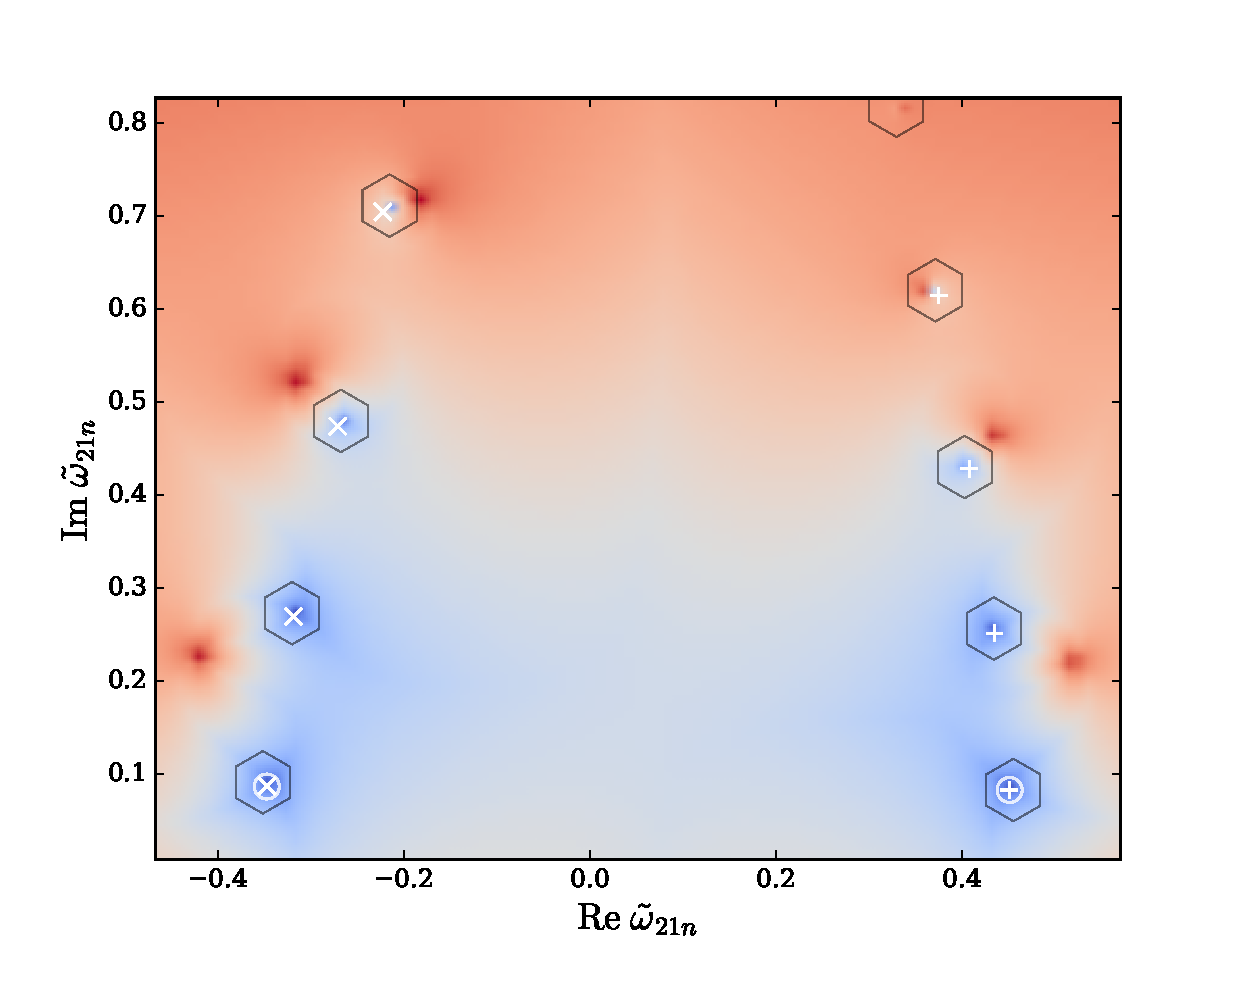
\includegraphics[width=\figfactor\textwidth]{leaver_example_chi0p68_l2m1.pdf} &
		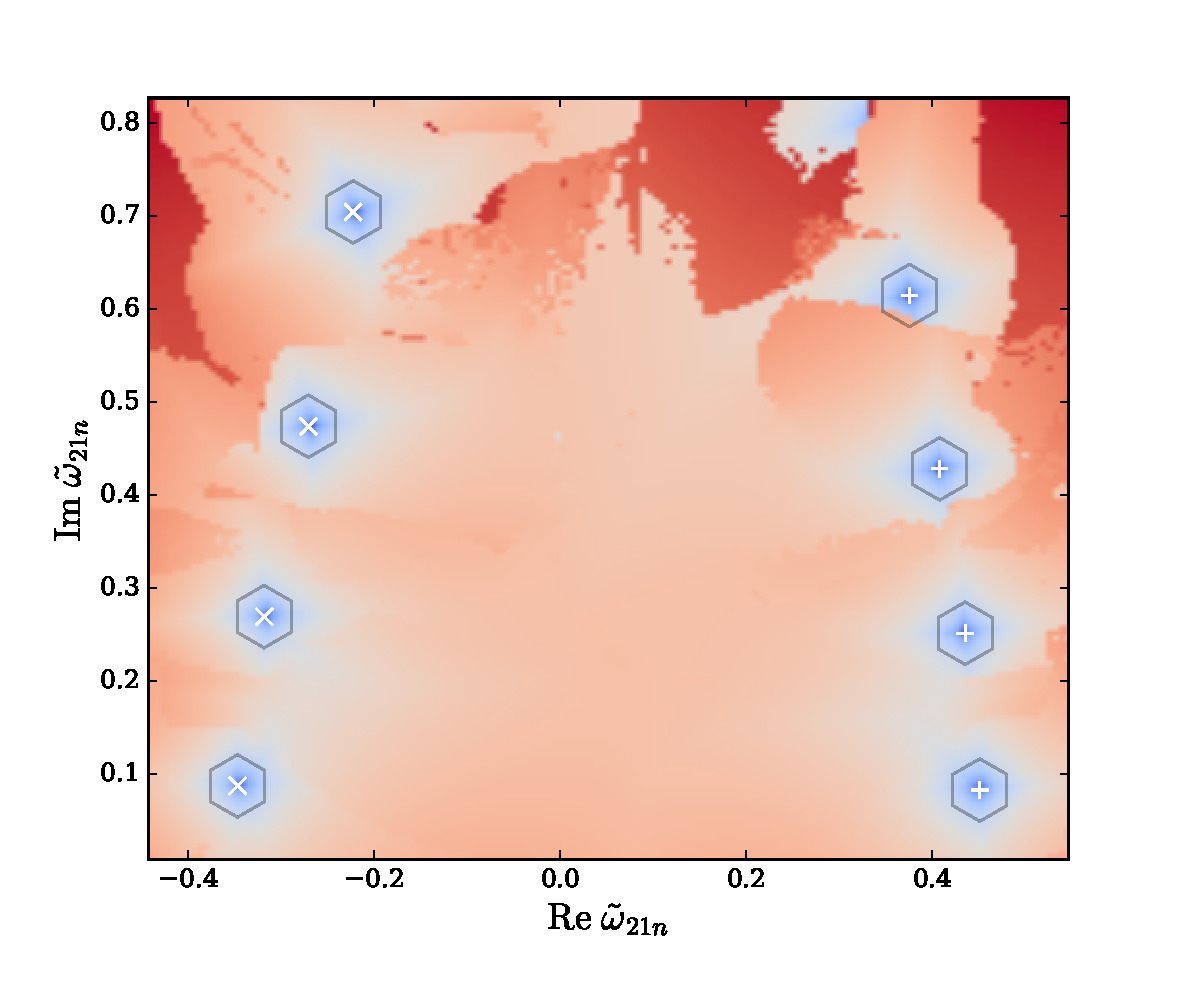
\includegraphics[width=\figfactor\textwidth]{leaver_example_chi0p68_l2m1_brute_r.pdf}
	\end{tabular}
	% 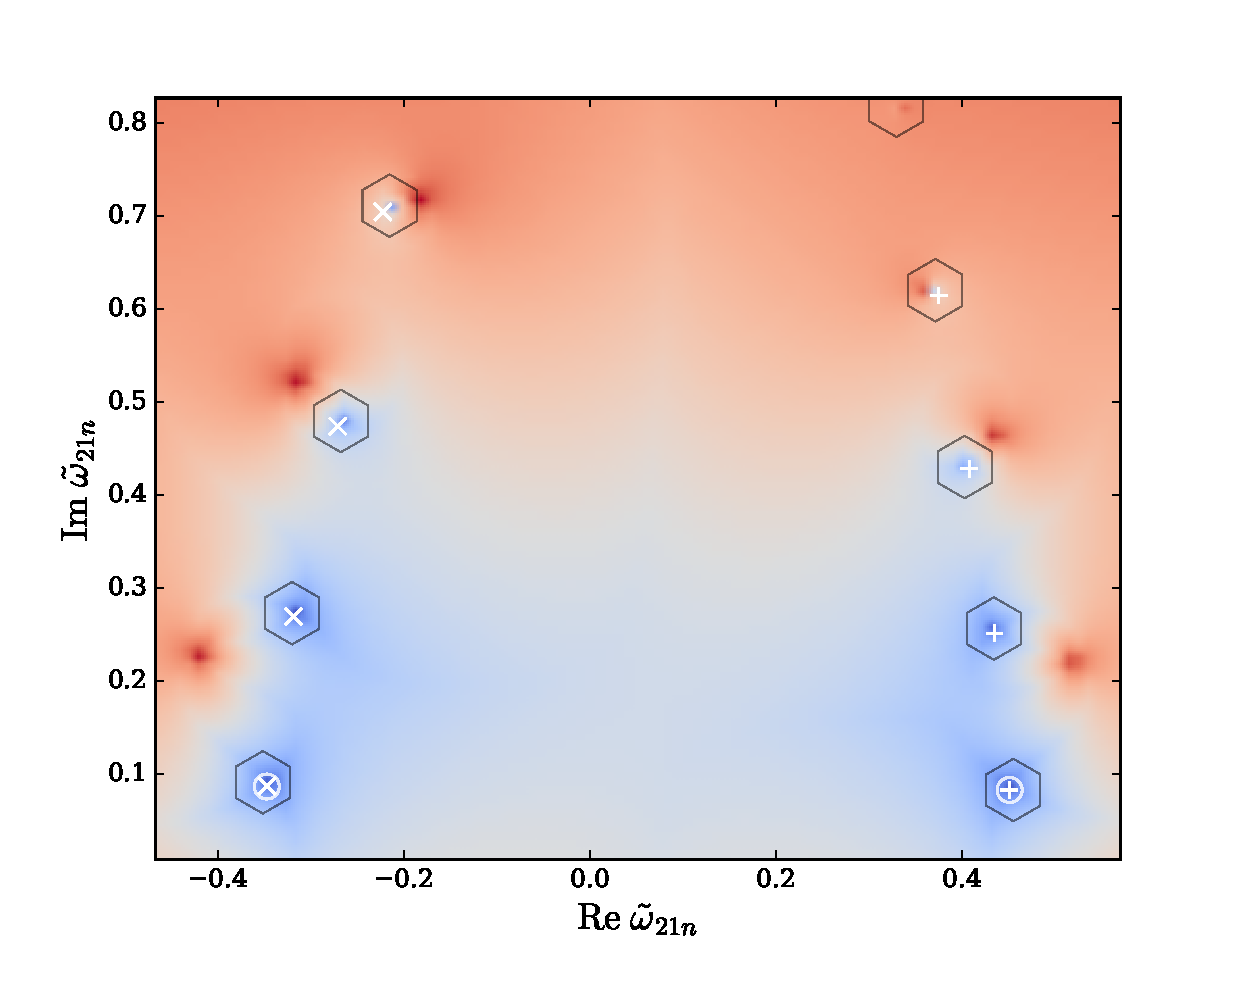
\includegraphics[width=\figfactor\textwidth]{leaver_example_chi0p68_l2m1.pdf}
	\caption{ Fits on leaver solutions }
	\label{fig:fitsanity}
\end{figure*}
%
There are two. This in conjunction with conjugate symmetry (\textit{i.e.} $m\rightarrow-m$), means that there are actually four. Got it??

\paragraph{\qnm{} Labeling Convention: --- } Note that we use a labeling convention for the \qnm{s} such that
%
	\begin{center}
		\begin{tabular}{ |l|c|c| }
			\hline
				Prograde 		&   $\j{} \ge 0$   & $\mathrm{sign}(\mathrm{re}(\omega_{lmn})) = \mathrm{sign}(m)$ \\
				Retrograde  &   $\j{}<0$   & $\mathrm{sign}(\mathrm{re}(\omega_{lmn})) = \mathrm{sign}(m)$ \\
			\hline
		\end{tabular}
	\end{center}
%
and the full wave solution is of the form
%
\begin{align}
	r\psi_k = &\sum_{k,\,\j{} \ge 0} \, A_k \, e^{ i \cw_k t} S_k(\j{}\CW_k,\theta,\phi) \, \\ \nonumber &+ \,  \sum_{k,\,\j{}<0} \, \left( A_k \, e^{i \cw_k t} \right)^* S_k(\j{}\CW_k^*,\theta,\phi) \; .
\end{align}
%
This differs from the convention used in \cite{Berti:2005ys}, which holds that $\j{}$ is always positive and
%
	\begin{center}
		\begin{tabular}{ |l|c|c| }
			\hline
				Prograde 		&   $\j{} \ge 0$   & $\mathrm{sign}(\mathrm{re}(\omega_{lmn})) = \mathrm{sign}(m)\;$ \\
				Retrograde  &   $\j{} \ge 0$   & $\mathrm{sign}(\mathrm{re}(\omega_{lmn})) = -\mathrm{sign}(m)$ \\
			\hline
		\end{tabular}
	\end{center}
%
making the full \textit{real-valued} waveform solution
%
\begin{align}
	r\psi_k = &\sum_{k} \, A_k \, e^{ i \CW_k t} S_k(\j{}\CW_k,\theta,\phi) \,  \\ \nonumber &+ \, \sum_{k} \, \left( A_k \, e^{i \CW_k t}  \right)^* S_k(\j{}\CW_k^*,\theta,\phi) \; .
\end{align}
%
Note that both conventions differ by a trivial relabeling of terms and result in the same \textit{real-valued} waveform.
%
\paragraph{Symmetry Relationships: --- } Note that the following symmetry relationships apply to the \qnm{} frequencies, $\cw_{lmn}$ and their related separation constants, $\SC_{lmn}$:
%
\begin{align}
	\cw_{l-mn} = - \cw_{lmn}^* \, , \quad \SC_{l-mn} = \SC_{lmn}^*
\end{align}
%
\paragraph{Different Perturbations: --- } In some extreme mass ratio cases, it appears that the frequency of the time domain waveform jumps from positive to negative during the merger-ringdown.
%
This the most valid interpretation for this scenario is that of the direction of the spin, $j(t) \rightarrow \j{}$, evolving drastically during this regime, in particular, going from positive to negative.
%
It seems that one should \textbf{not} interpret the two frequencies in this case as being simply a superposition of $m>0$ and $m<0$ as the transition between spin orientations is not trivially the transition in dominance between one \qnm{} and the other.
%
The related question is \textbf{\textit{What does the spin evolution look like for these cases?}}
%
Upon further thought, there appear to be two core scenarios:
%
\begin{itemize}
	\item[(S1)] The direction of $\hat{j}(t)$ inverts during the system's evolution, leaving the final perturbation to be dominantly prograde relative to $\hat{j}_f=-\hat{j}_i$.
	\item[(S2)] The direction of $\hat{j}(t)$ stays ``fixed'' throughout the system's evolution, but the perturbation transitions from prograde to be dominantly retrograde relative to $\hat{j}_f$.
\end{itemize}
%
\paragraph{\ul{To-Do List}: --- }
%
\begin{itemize}
	%
	\item Add plot of QNM frequency fit points on 2D colormap of \texttt{leaver\_workfunction} at fixed separation constant to further illustrate.
	\item \textbf{Implement as full waveform model in python before continuing!}
	\begin{itemize}
		%\item[$\circ$] Use MATLAB to write python lambda function for QNM amplitudes and frequencies.
		%\item[$\circ$] Include above lambda functions in python model for RD.
		\item[$\circ$] Make polynomial model for separation constants.
		\item[$\circ$] Were/Are phases of frequencies and separation constants consistent for spheroidal harmonic calculation?
	\end{itemize}
	\item The model has been changed so that the overall eta dependence is not dependent on the overtone number.
	\item Recent work in analytic perturbation theory suggests, if I recall correctly, that the overtones may be a guage artifact. \textbf{Is this a correct statement and does it apply here?}
	\item There seems to be a problem with the current $(2,1,0)$ \qnm{} frequency: when using the imaginary part for $\SCc_k$ fitting, the nearly extremal Kerr behavior (\textit{i.e.} it derivatives) seems to be inconsistent with the numerical data.
\end{itemize}

}
% %%%%%%%%%%%%%%%%%%%%%%%%%%%%%%%%%%%%%%%%%%%%%%%% %

%
\appendix

%
\section{A Complex Polynomial Model for Dimensionless QNM Frequencies}
\label{app:cwmodel}
%
\par While it is possible to refer to the work of Leaver and others to numerically compute the \qnm{} frequencies of Kerr, it is more convenient to utilize a closed form function, in particular, a fit to the numerical values, for the same task.
%
\begin{figure}[htb]
	\vspace{0.15cm}
	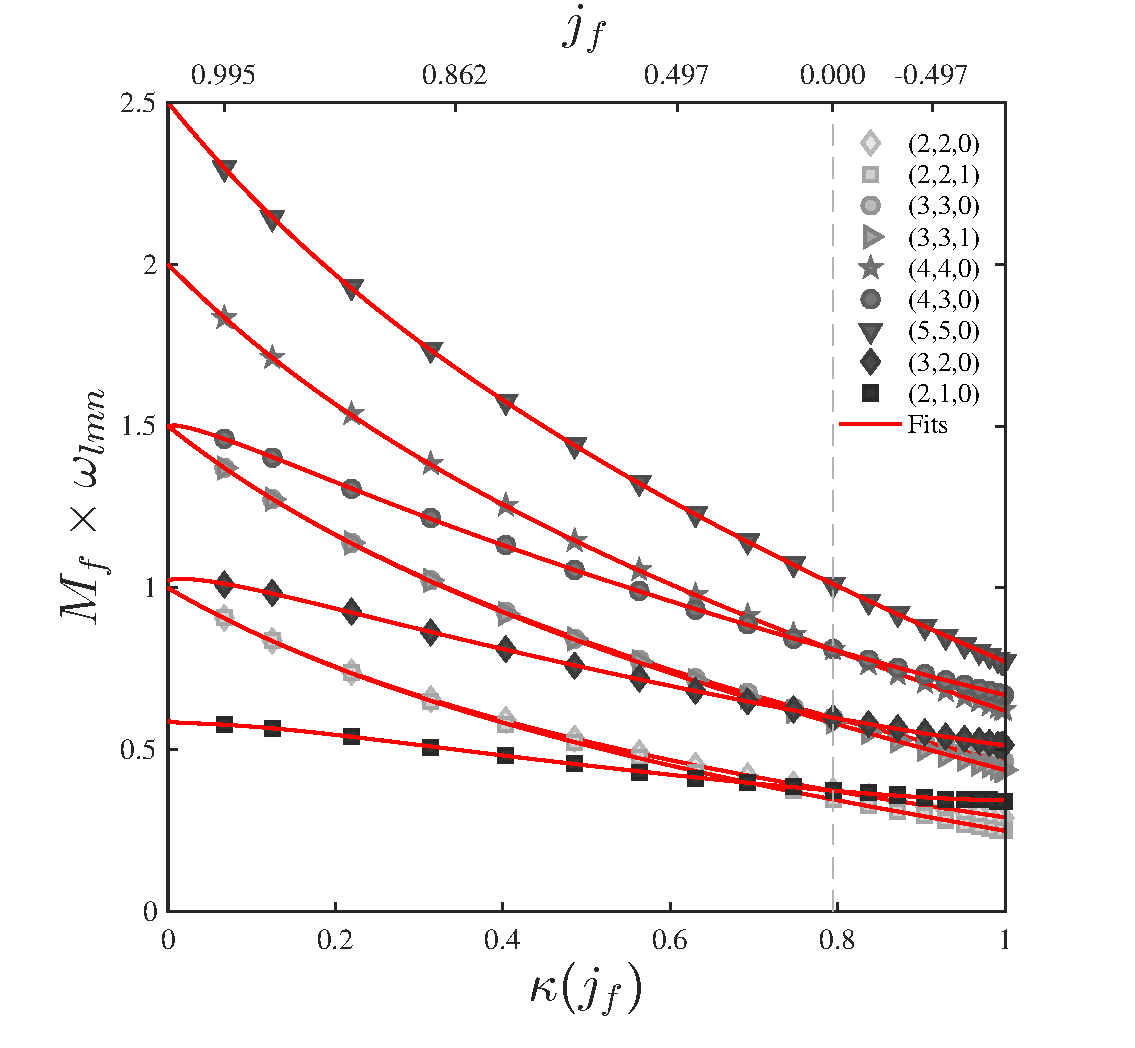
\includegraphics[width=\figfactor\textwidth]{fits_w.pdf}
	\caption{ Fits of dimensionless \qnm{} central frequencies (solid lines) along with select numerical values (grey markers) computed using Leaver's method \cite{Leaver85}. Before the application of $\kappa(\j{})$, points are spaced between -\CwFitCalibrationRegion and \CwFitCalibrationRegion according to \CwFitCalibrationRegion times the $\sin$ of a fiducial angle which is uniformly spaced between $-\pi/2$ and $\pi/2$. Values of $\j{}$ are shown in the upper axis for $\kappa$ at $l=m$. The grey dashed line marks the value of $\kappa$ where $\j{}=0$.}
	\label{fig:wfits}
\end{figure}
% %
% \begin{figure}[htb]
% 	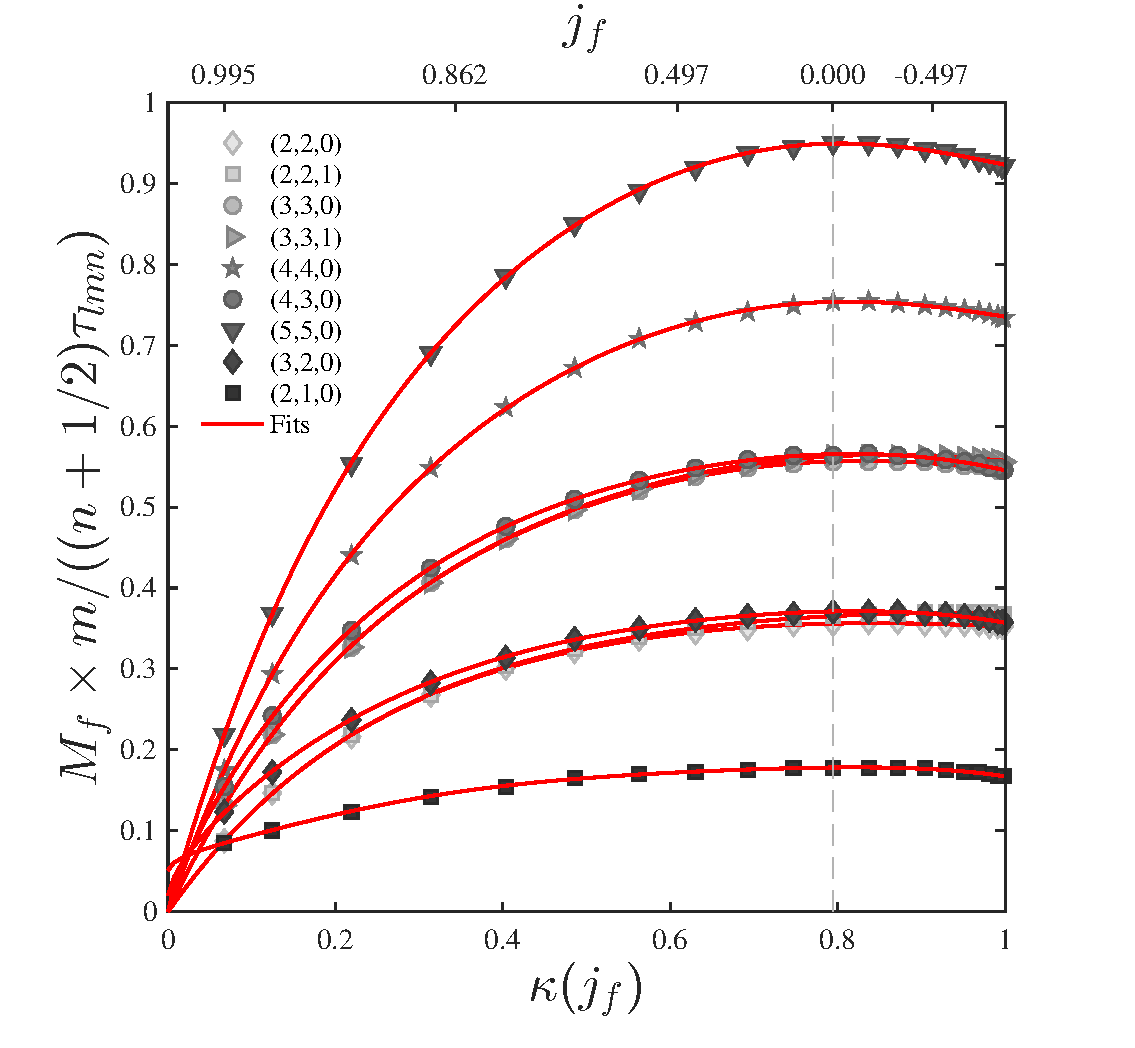
\includegraphics[width=\figfactor\textwidth]{fits_tau.pdf}
% 	\caption{ Fits. }
% 	\label{fig:taufits}
% \end{figure}
% %
% \begin{figure}[htb]
% 	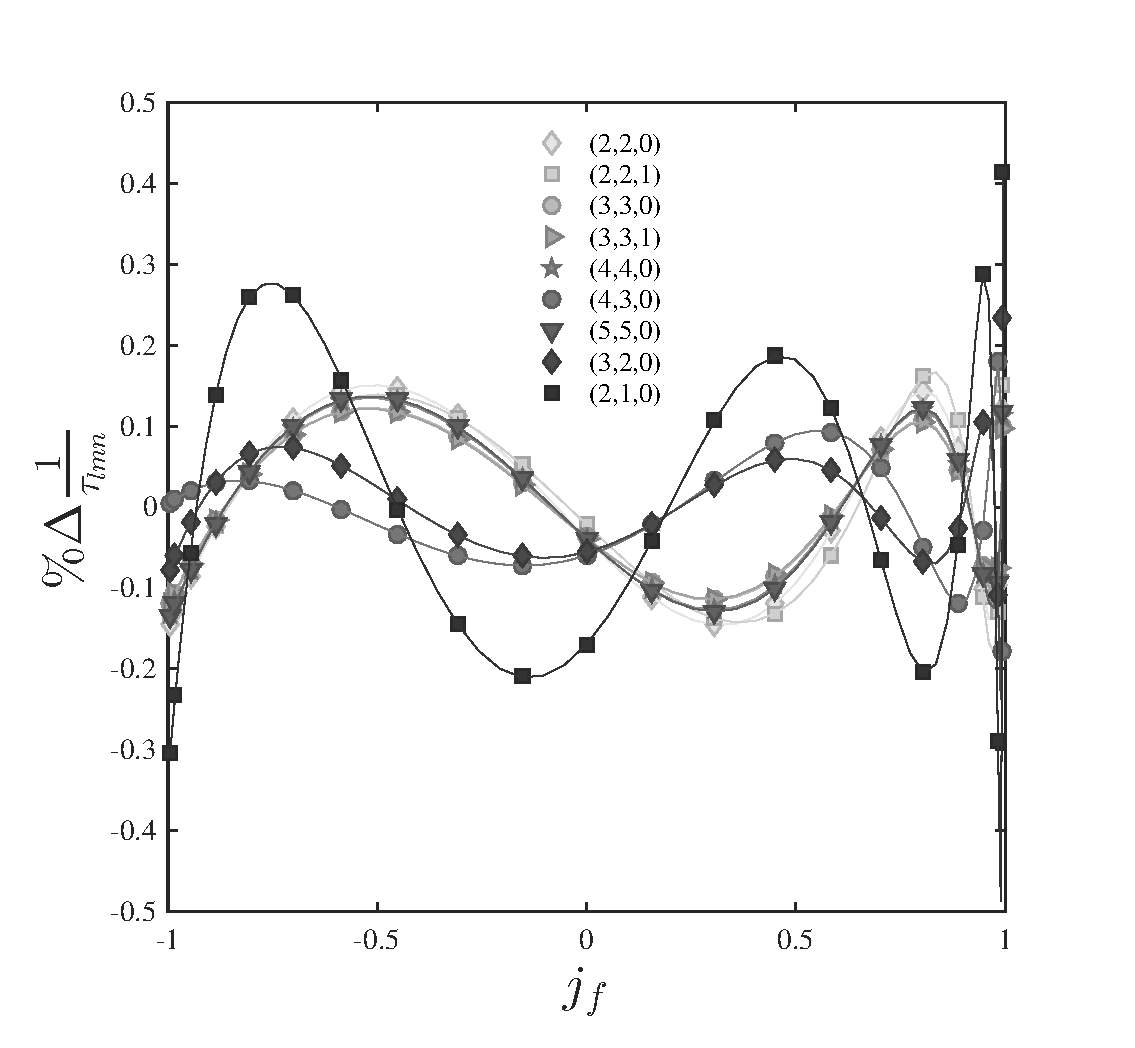
\includegraphics[width=\figfactor\textwidth]{res_tau.pdf}
% 	\caption{ Residuals. }
% 	\label{fig:taures}
% \end{figure}
% %
% \begin{figure}[htb]
% 	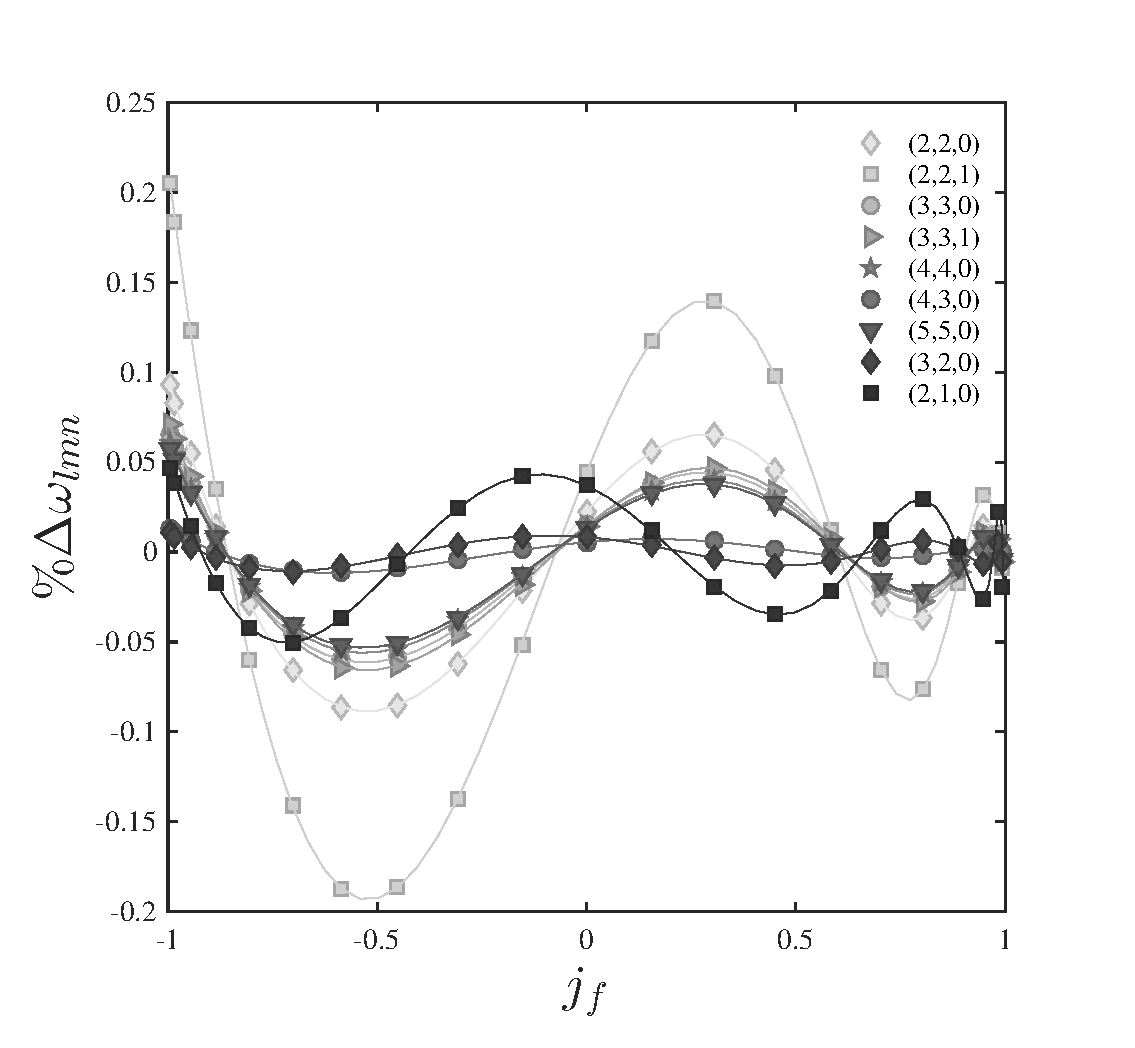
\includegraphics[width=\figfactor\textwidth]{res_w.pdf}
% 	\caption{ Residuals. }
% 	\label{fig:wres}
% \end{figure}
%
This section details such a fit for the dimensionless \qnm{} frequency, $\CW_{k}$ (See \ceqn{eq:Mw}), as well as brief comparisons with similar fits in the literature.
%
Previous fits separately model the real and imaginary parts of $\CW_{k}$ on $0 \leq \j{} < 1$, and treat prograde and retrograde \qnm{} disjointly \cite{Berti:2005ys}.
%
Here we recognize that the retrograde frequencies may be associated with negative \bh{} spin (\textit{e.g.} one pointing oppositely of an initial orbital angular momentum direction).
%
This point illuminates that the prograde and retrograde \qnm{} frequencies are continuously connected as $\j{}$ transitions from positive to negative.
%
We therefore construct a model, $\CW_{k}(\j{})$, where the domain, $\j{}$, ranges from $-1$ to $1$.
%

% \begin{figure*}[htb]
% 	\begin{tabular}{cc}
% 		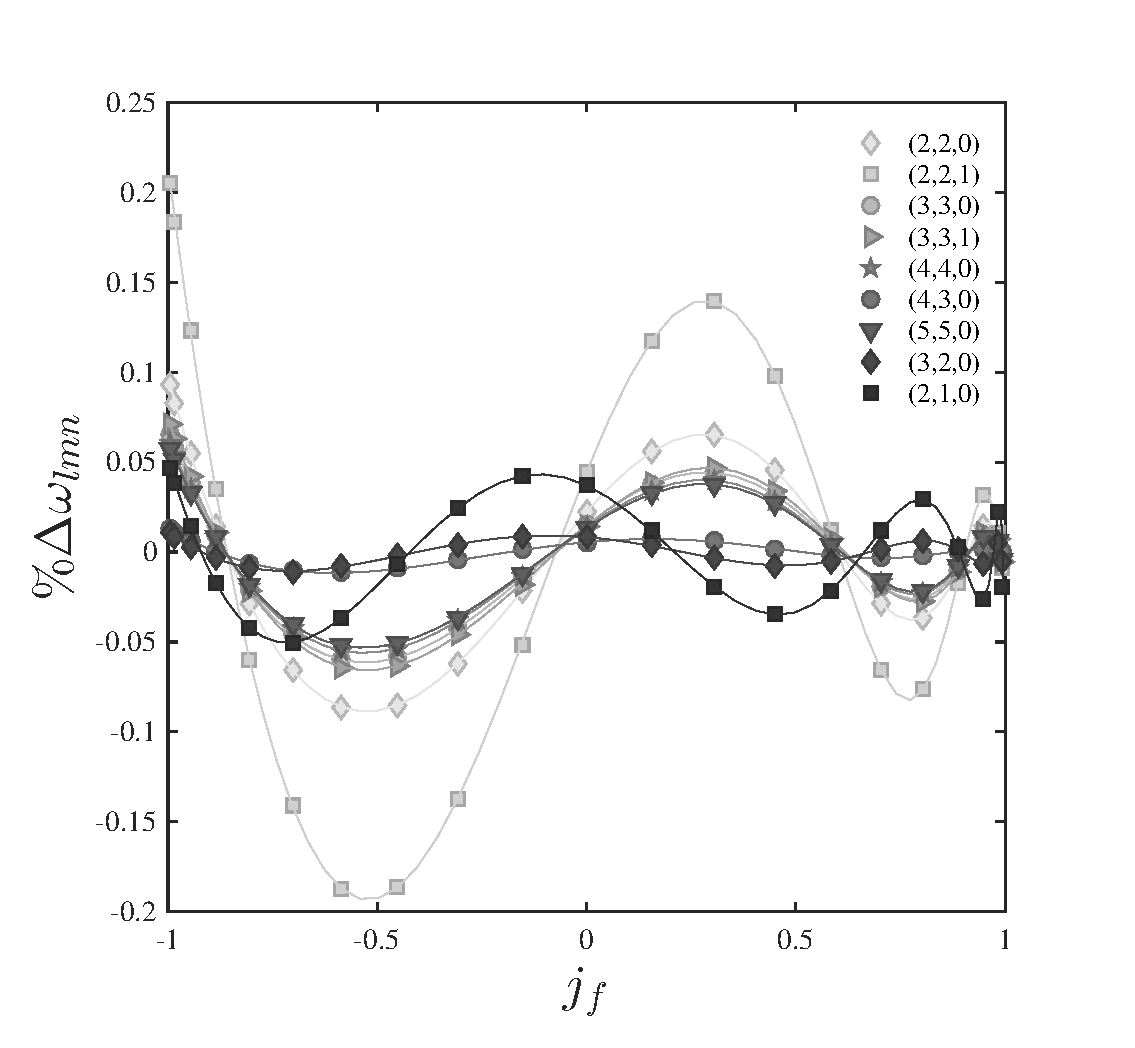
\includegraphics[width=\figfactor\textwidth]{res_w.pdf} &
% 		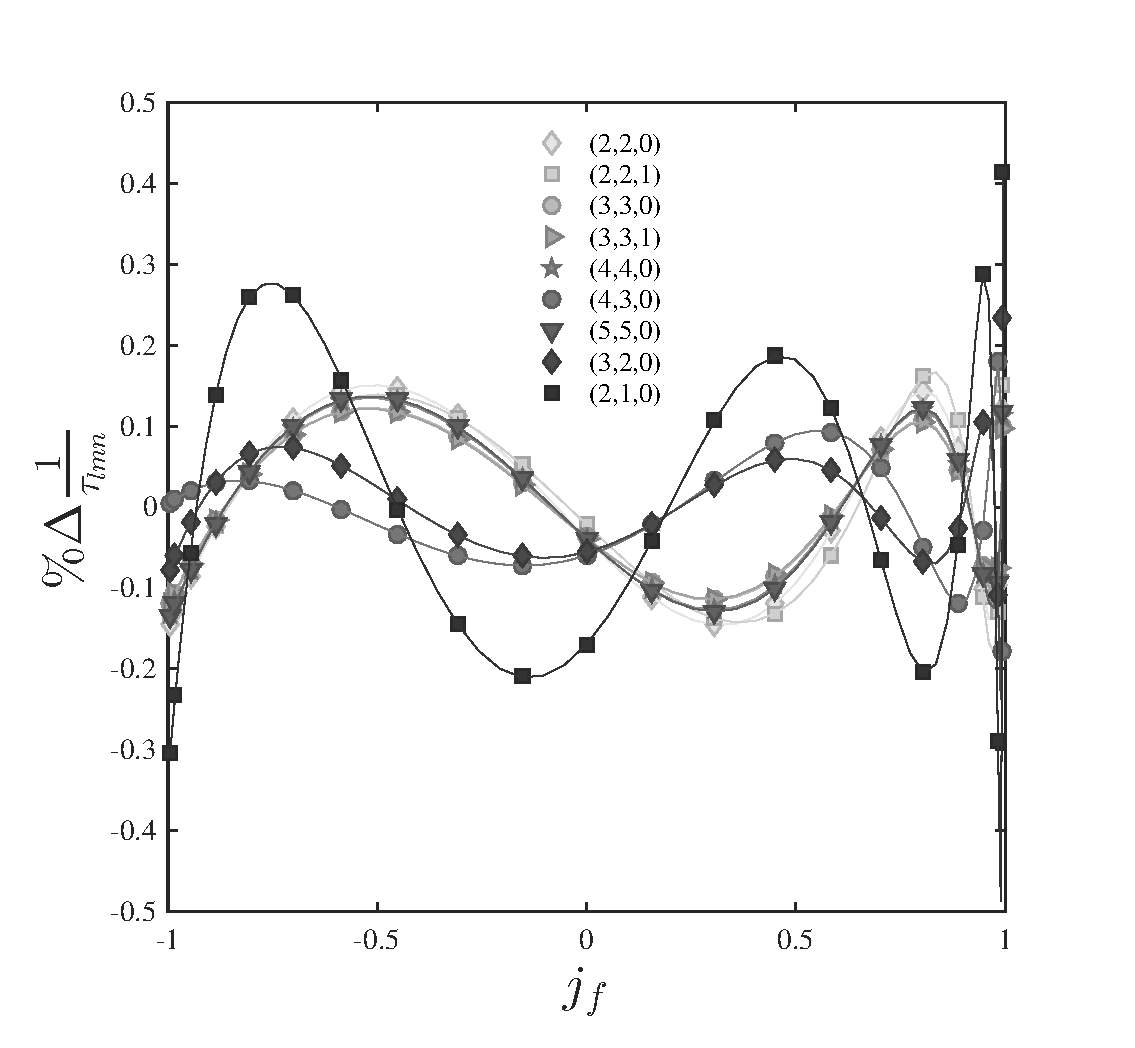
\includegraphics[width=\figfactor\textwidth]{res_tau.pdf}
% 	\end{tabular}
% 	\caption{ Percentage residuals of \qnm{} frequency model. \textit{Left Panel}: Percentage residuals for central frequency, $\omega_{lmn}$. \textit{Right Panel}: Percentage residuals for the inverse decay rate, $1/\tau_{lmn}$. See \eqns{eq:percw}{eq:perctau} for the definitions of $\%\Delta\omega_{lmn}$ and $\%\Delta\frac{1}{\tau_{lmn}}$. \red{COMBINE PLOTS} }
% 	\label{fig:cwres}
% \end{figure*}

\begin{figure}[htb]
	{\hspace{0cm}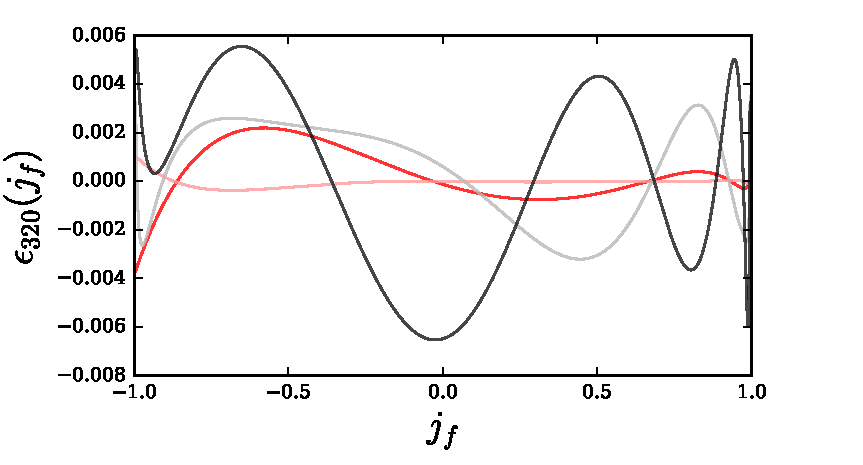
\includegraphics[width=\figfactor\textwidth]{test_python_fit_equations_l3m2n0.pdf}}
	\caption{ Residuals of Leaver's constraint equations for \qnm{} solutions to Teukolsky's equations. \red{The equations are ... the quantities are ...} }
	\label{fig:lvrres}
\end{figure}

%
\par Furthermore, noting that each \qnm{} frequency, $\CW_k$, changes rapidly near $\j{} \approx 1$, we chose to perform a domain mapping, $\kappa(\j{})$, prior to fitting.
%
We find that defining $\kappa(\j{})$ as
%
\begin{align}
	\kappa(\j{}) \; = \; \left( \log_3 [ 2 - \j{}  ] \right)^{ 1/(|s| - |m| + l) } \quad \text{($s=-2$)} \; .
		\label{eq:jf_map}
\end{align}
%
effectively maps $(-1,1)$ to $(1,0)$ while simultaneously simplifying the behavior of each $\CW_k$ near $\j{}=1$.
%
This simplification corresponds to the largely linear and parabolic behavior of the \qnm{} frequencies shown in \fig{fig:wfits}.
%
\par After applying \eqn{eq:jf_map} to $\j{}$, we find that all of the \qnm{} frequencies considered here are extremely well modeled by a polynomial of order $4$ whose coefficients are complex (See \ceqns{eq:cw_fit_1}{eq:cw_fit_9}).
%
Information from the near-extremal Kerr perturbation theory has been utilized (\textit{e.g.} \cite{Dias:2015wqa,Zimmerman:2015rua,Zimmerman:2015trm,Yang:2012pj}).
%
In particular, \eqns{eq:cw_fit_1}{eq:cw_fit_9} have been constructed to be consistent with the zero damped mode (ZDM) branch of the nearly extremal Kerr limit where, as $\j{} \rightarrow 0$, the real part of the complex \qnm{} frequency tends to $m/2$, the critical frequency for super-radiance.
%
Therefore the fitting formula take on the generalized form
%
\begin{align}
	\label{eq:cw_ansatz}
	\CW_{lmn}(\kappa) \; = \; m/2 \, + \, \sum_{p} \, g_p \, \kappa^p \; ,
\end{align}
%
where $g_p$ are complex valued.
%
This fitting ansatz aims to reproduce the ZDM branch of the Kerr spectrum.
%
The damped-mode branch of the nearly extremal Kerr spectrum is not treated in the fit.
%
\begin{widetext}
	\red{
		\begin{align}
	\label{eq:cw_fit_1}
	\CW_{220}(\kappa) \; &= \;\, 1.0 \, + \, \kappa \, (1.5578 e^{2.9031 i}\, + \, 1.9510  e^{5.9210 i} \kappa\, + \, 2.0997  e^{2.7606 i} \kappa ^ 2\, + \, 1.4109  e^{5.9143 i} \kappa ^ 3\, + \, 0.4106  e^{2.7952 i} \kappa ^ 4 \, )  \\ 
	\label{eq:cw_fit_2}
	\CW_{221}(\kappa) \; &= \;\, 1.0 \, + \, \kappa \, (1.8709 e^{2.5112 i}\, + \, 2.7192  e^{5.4250 i} \kappa\, + \, 3.0565  e^{2.2857 i} \kappa ^ 2\, + \, 2.0531  e^{5.4862 i} \kappa ^ 3\, + \, 0.5955  e^{2.4225 i} \kappa ^ 4 \, )  \\ 
	\label{eq:cw_fit_3}
	\CW_{330}(\kappa) \; &= \;\, 1.5 \, + \, \kappa \, (2.0957 e^{2.9650 i}\, + \, 2.4696  e^{5.9967 i} \kappa\, + \, 2.6655  e^{2.8176 i} \kappa ^ 2\, + \, 1.7584  e^{5.9327 i} \kappa ^ 3\, + \, 0.4991  e^{2.7817 i} \kappa ^ 4 \, )  \\ 
	\label{eq:cw_fit_4}
	\CW_{331}(\kappa) \; &= \;\, 1.5 \, + \, \kappa \, (2.3391 e^{2.6497 i}\, + \, 3.1399  e^{5.5525 i} \kappa\, + \, 3.5916  e^{2.3472 i} \kappa ^ 2\, + \, 2.4490  e^{5.4435 i} \kappa ^ 3\, + \, 0.7004  e^{2.2830 i} \kappa ^ 4 \, )  \\ 
	\label{eq:cw_fit_5}
	\CW_{440}(\kappa) \; &= \;\, 2.0 \, + \, \kappa \, (2.6589 e^{3.0028 i}\, + \, 2.9783  e^{6.0510 i} \kappa\, + \, 3.2184  e^{2.8775 i} \kappa ^ 2\, + \, 2.1276  e^{5.9897 i} \kappa ^ 3\, + \, 0.6034  e^{2.8300 i} \kappa ^ 4 \, )  \\ 
	\label{eq:cw_fit_6}
	\CW_{430}(\kappa) \; &= \;\, 1.5 \, + \, \kappa \, (0.2050 e^{0.5953 i}\, + \, 3.1033  e^{3.0162 i} \kappa\, + \, 4.2361  e^{6.0388 i} \kappa ^ 2\, + \, 3.0289  e^{2.8262 i} \kappa ^ 3\, + \, 0.9084  e^{5.9152 i} \kappa ^ 4 \, )  \\ 
	\label{eq:cw_fit_7}
	\CW_{550}(\kappa) \; &= \;\, 2.5 \, + \, \kappa \, (3.2405 e^{3.0279 i}\, + \, 3.4906  e^{6.0888 i} \kappa\, + \, 3.7470  e^{2.9212 i} \kappa ^ 2\, + \, 2.4725  e^{6.0365 i} \kappa ^ 3\, + \, 0.6994  e^{2.8766 i} \kappa ^ 4 \, )  \\ 
	\label{eq:cw_fit_8}
	\CW_{320}(\kappa) \; &= \;\,1.0225 e^{0.0049 i}\, + \, 0.2473  e^{0.6653 i} \kappa\, + \, 1.7047  e^{3.1383 i} \kappa ^ 2\, + \, 0.9460  e^{0.1632 i} \kappa ^ 3\, + \, 1.5319  e^{5.7036 i} \kappa ^ 4\\ \nonumber
	&\hspace{255pt}\, + \, 2.2805  e^{2.6852 i} \kappa ^ 5\, + \, 0.9215  e^{5.8417 i} \kappa ^ 6 \\ 
	\label{eq:cw_fit_9}
	\CW_{210}(\kappa) \; &= \;\,0.5891 e^{0.0435 i}\, + \, 0.1890  e^{2.2899 i} \kappa\, + \, 1.1501  e^{5.8101 i} \kappa ^ 2\, + \, 6.0459  e^{2.7420 i} \kappa ^ 3\, + \, 11.1263  e^{5.8441 i} \kappa ^ 4\\ \nonumber
	&\hspace{255pt}\, + \, 9.3471  e^{2.6694 i} \kappa ^ 5\, + \, 3.0384  e^{5.7915 i} \kappa ^ 6
\end{align}

	}
\end{widetext}
%
\par \fig{fig:wfits} shows the fits and related numerical data for all \qnm{s} considered here.
%
\fig{fig:lvrres} shows the related (percentage) residual errors over the calibration region, with
%
\begin{align}
	\%\Delta \omega_k \; = \; \%\Delta M_f \omega_k \; = \; 100 \times ( \omega^{\mathrm{Fit}}_k - \omega_k ) / |\omega_k|
	\label{eq:percw}
\end{align}
%
and
%
\begin{align}
	\%\Delta (1/\tau_k) \; = \; \%\Delta (M_f / \tau_k) \; = \; 100 \times ( 1/\tau^{\mathrm{Fit}}_k - 1/\tau_k ) / (1/\tau_k) \; .
	\label{eq:perctau}
\end{align}
%
While \NumCalibrationPoints calibration points were used for the fit, only \NumCalibrationPointsPlotted points are shown for clarity.
%
As the model encapsulated by \eqns{eq:cw_fit_1}{eq:cw_fit_9} has only been calibrated for $\j{}$ on $(-\CwFitCalibrationRegion,\CwFitCalibrationRegion)$, nearly extremal spin features of the \qnm{} frequencies, such as zero damping branching (\textit{e.g} \cite{Yang:2012pj} ), are \textit{not} captured by the model presented here.
%
\par The model presented in this section applies to the $-m$ \qnm{s} according to
%
\begin{align}
	\CW_{lmn}^* \; = \; -\CW_{lm'n}^* \text{, where } m' \; = \; -m \;,
	\label{eq:cwsymm}
\end{align}
%
and $*$ denotes complex conjugation.
%
\par Moreover, it is also of practical use to note that one may trivially obtain dimentionful \qnm{} frequencies by scaling by the \bh{} mass: $$\cw_k \; = \; \CW_k / M_f\;.$$
%
In practice, $\cw_k$ (\textit{i.e.} $\cw_{lmn}$) are most often used (\textit{e.g.} as in \ceqn{eq:psi4pt}).

%
\section{A Complex Polynomial Model for QNM Separation Constants}
%
\par The \qnm{} separation constants are needed in order to compute the spheroidal harmonic functions according to \red{[Add Equation]}.
%
Here, we use the same domain mapping as in \sec{app:cwmodel}.
%
In addition we consider the complex valued separation constant's real and imaginary parts separately
%
\begin{align}
	\label{eq:scrc}
	\SC_k \, = \, \SC^\mathrm{r}_k \, + \, i\,\SC^\mathrm{c}_k \; .
\end{align}
%
For $\SC^\mathrm{r}_k$, a direct polynomial fit is applied.
%
For $\SC^\mathrm{c}_k$, where there are natural roots (e.g. at $\j{}=0$, and in the case of the modes with zero damping as $\j{}\rightarrow1$, $\j{}=1$), we scale away the simplest polynomial form associated with these roots before fitting, and rescale afterwards.
%
This has the effect of simplifying the fit and enforcing strict root locations.
%
Although performed separately, the two fits are combined according to \eqn{eq:scrc}.
%
The resulting fit equations are by \eqns{eq:cw_fit_1}{eq:cw_fit_9}.
%
\blue{Note that the number of significant digits shown here is limited for brevity. Fitting parameters at full precision may be found on github.}
%
\begin{widetext}
	\red{
		\begin{align}
	\label{eq:cw_fit_1}
	\SC_{220}(\kappa) \; &= \;0.5526 e^{0.0000 i}\, + \, 6.5427  e^{0.2444 i} \kappa\, + \, 5.9466  e^{3.8841 i} \kappa ^ 2\, + \, 5.3930  e^{1.0165 i} \kappa ^ 3\, + \, 3.5870  e^{4.5340 i} \kappa ^ 4\\ \nonumber
	&\quad\, + \, 1.3686  e^{1.5708 i} \kappa ^ 5\, + \, 0.1852  e^{4.7124 i} \kappa ^ 6 \\ 
	\label{eq:cw_fit_2}
	\SC_{221}(\kappa) \; &= \;0.5523 e^{0.0000 i}\, + \, 7.9407  e^{0.6408 i} \kappa\, + \, 12.5557  e^{4.4198 i} \kappa ^ 2\, + \, 13.6852  e^{1.4804 i} \kappa ^ 3\, + \, 10.4388  e^{4.7260 i} \kappa ^ 4\\ \nonumber
	&\quad\, + \, 4.2073  e^{1.5708 i} \kappa ^ 5\, + \, 0.7623  e^{4.7124 i} \kappa ^ 6 \\ 
	\label{eq:cw_fit_3}
	\SC_{210}(\kappa) \; &= \;3.1009 e^{6.2582 i}\, + \, 2.6921  e^{1.9585 i} \kappa\, + \, 16.5858  e^{4.9842 i} \kappa ^ 2\, + \, 57.8409  e^{1.6372 i} \kappa ^ 3\, + \, 118.2176  e^{4.7267 i} \kappa ^ 4\\ \nonumber
	&\quad\, + \, 135.9399  e^{1.5708 i} \kappa ^ 5\, + \, 82.8174  e^{4.7124 i} \kappa ^ 6\, + \, 20.8517  e^{1.5708 i} \kappa ^ 7 \\ 
	\label{eq:cw_fit_4}
	\SC_{330}(\kappa) \; &= \;5.7047 e^{0.0000 i}\, + \, 7.9443  e^{0.1804 i} \kappa\, + \, 6.5510  e^{3.7793 i} \kappa ^ 2\, + \, 6.3142  e^{0.9386 i} \kappa ^ 3\, + \, 4.8121  e^{4.4691 i} \kappa ^ 4\\ \nonumber
	&\quad\, + \, 2.3893  e^{1.5708 i} \kappa ^ 5\, + \, 0.4808  e^{4.7124 i} \kappa ^ 6 \\ 
	\label{eq:cw_fit_5}
	\SC_{331}(\kappa) \; &= \;5.7032 e^{0.0000 i}\, + \, 8.9493  e^{0.4983 i} \kappa\, + \, 12.7053  e^{4.3177 i} \kappa ^ 2\, + \, 15.6353  e^{1.3939 i} \kappa ^ 3\, + \, 14.1906  e^{4.6691 i} \kappa ^ 4\\ \nonumber
	&\quad\, + \, 7.3324  e^{1.5708 i} \kappa ^ 5\, + \, 1.5370  e^{4.7124 i} \kappa ^ 6 \\ 
	\label{eq:cw_fit_6}
	\SC_{320}(\kappa) \; &= \;8.1854 e^{6.2760 i}\, + \, 1.5519  e^{1.7909 i} \kappa\, + \, 8.9465  e^{5.1868 i} \kappa ^ 2\, + \, 28.6605  e^{1.6366 i} \kappa ^ 3\, + \, 60.7779  e^{4.7211 i} \kappa ^ 4\\ \nonumber
	&\quad\, + \, 72.1324  e^{1.5708 i} \kappa ^ 5\, + \, 45.3812  e^{4.7124 i} \kappa ^ 6\, + \, 11.8471  e^{1.5708 i} \kappa ^ 7 \\ 
	\label{eq:cw_fit_7}
	\SC_{440}(\kappa) \; &= \;13.0529 e^{0.0000 i}\, + \, 9.2346  e^{0.1418 i} \kappa\, + \, 7.0905  e^{3.6918 i} \kappa ^ 2\, + \, 6.4671  e^{0.8925 i} \kappa ^ 3\, + \, 4.9691  e^{4.4385 i} \kappa ^ 4\\ \nonumber
	&\quad\, + \, 2.6230  e^{1.5708 i} \kappa ^ 5\, + \, 0.5817  e^{4.7124 i} \kappa ^ 6 \\ 
	\label{eq:cw_fit_8}
	\SC_{430}(\kappa) \; &= \;15.2887 e^{0.0000 i}\, + \, 0.7530  e^{0.2205 i} \kappa\, + \, 3.6494  e^{0.6164 i} \kappa ^ 2\, + \, 8.0253  e^{4.8276 i} \kappa ^ 3\, + \, 12.4721  e^{1.6733 i} \kappa ^ 4\\ \nonumber
	&\quad\, + \, 10.3028  e^{4.7124 i} \kappa ^ 5\, + \, 3.5289  e^{1.5708 i} \kappa ^ 6 \\ 
	\label{eq:cw_fit_9}
	\SC_{550}(\kappa) \; &= \;22.5229 e^{0.0000 i}\, + \, 10.4414  e^{0.1161 i} \kappa\, + \, 7.7971  e^{3.6125 i} \kappa ^ 2\, + \, 6.5999  e^{0.8379 i} \kappa ^ 3\, + \, 4.9037  e^{4.4055 i} \kappa ^ 4\\ \nonumber
	&\quad\, + \, 2.5991  e^{1.5708 i} \kappa ^ 5\, + \, 0.5899  e^{4.7124 i} \kappa ^ 6
\end{align}

	}
\end{widetext}

%
\section{A Model for the Spheroidal Harmonic Normalization Constants}

%
It is useful to be able to normalize the spheroidal harmonic functions.
%
While the normailzation constants reduce to those of the spin -2 spherical harmonics for $\j{}=0$, an analytic form for all spins is not known at the time of this publication.
%
Therefore, we present a polynomial fit for the normalization constants for the \qnm{} used here.
%
\par The spheroidal harmonic functions, $\mathcal{S}_{k}(\j{}M_f\cw{}_k, \theta, \phi)$, were calculated according to Leaver's solution with no additional scaling \cite{Leaver85}.
%
We define the normalization constant, $\mathcal{C}_k$, such that
%
\begin{align}
	\label{eq:slm_norm}
	\int_{\Omega} \, \mathcal{S}^*_k \, \mathcal{S}_k \, d\Omega \; = \; 1
\end{align}
%
We find that the resulting normalization constants are well captured, with all residual errors less than $0.5\%$, by \eqns{eq:cc_fit_1}{eq:cc_fit_9}.
%
\begin{widetext}
	\begin{align}
	\label{eq:cc_fit_1}
	\CC_{220}(\kappa) \; &= \;7.8637\, - \, 3.6145 \kappa\, + \, 3.4900 \kappa ^ 2\, - \, 2.2935 \kappa ^ 3\, + \, 0.7443 \kappa ^ 4 \\ 
	\label{eq:cc_fit_2}
	\CC_{221}(\kappa) \; &= \;7.8630\, - \, 3.5987 \kappa\, + \, 2.8846 \kappa ^ 2\, - \, 0.9274 \kappa ^ 3\, - \, 0.0445 \kappa ^ 4 \\ 
	\label{eq:cc_fit_3}
	\CC_{330}(\kappa) \; &= \;3.5163\, + \, 0.1650 \kappa\, + \, 1.3011 \kappa ^ 2\, - \, 0.8362 \kappa ^ 3\, + \, 0.8202 \kappa ^ 4 \\ 
	\label{eq:cc_fit_4}
	\CC_{331}(\kappa) \; &= \;3.5153\, + \, 0.1929 \kappa\, + \, 0.9681 \kappa ^ 2\, - \, 0.0055 \kappa ^ 3\, + \, 0.2498 \kappa ^ 4 \\ 
	\label{eq:cc_fit_5}
	\CC_{440}(\kappa) \; &= \;1.7539\, + \, 1.0011 \kappa\, + \, 1.5550 \kappa ^ 2\, - \, 1.2234 \kappa ^ 3\, + \, 1.6462 \kappa ^ 4 \\ 
	\label{eq:cc_fit_6}
	\CC_{550}(\kappa) \; &= \;0.9135\, + \, 0.8957 \kappa\, + \, 2.5440 \kappa ^ 2\, - \, 2.8244 \kappa ^ 3\, + \, 3.2814 \kappa ^ 4 \\ 
	\label{eq:cc_fit_7}
	\CC_{210}(\kappa) \; &= \;3.0439\, - \, 0.0688 \kappa\, + \, 0.8767 \kappa ^ 2\, - \, 3.9221 \kappa ^ 3\, + \, 8.5963 \kappa ^ 4\, - \, 8.5220 \kappa ^ 5\, + \, 3.3115 \kappa ^ 6 \\ 
	\label{eq:cc_fit_8}
	\CC_{320}(\kappa) \; &= \;0.7485\, - \, 0.0816 \kappa\, + \, 1.0375 \kappa ^ 2\, - \, 3.2793 \kappa ^ 3\, + \, 7.2458 \kappa ^ 4\, - \, 7.4132 \kappa ^ 5\, + \, 3.0606 \kappa ^ 6 \\ 
	\label{eq:cc_fit_9}
	\CC_{430}(\kappa) \; &= \;0.3954\, - \, 0.0992 \kappa\, + \, 1.5285 \kappa ^ 2\, - \, 5.0993 \kappa ^ 3\, + \, 10.9565 \kappa ^ 4\, - \, 10.9991 \kappa ^ 5\, + \, 4.5221 \kappa ^ 6
\end{align}

\end{widetext}


%
\section{Fitting Formula for QNM Complex Amplitudes}

Here we list fitting formula for various \pn{} scaled \qnm{} amplitudes in the Spherical basis.

\red{
\begin{widetext}
	\begin{center}
		%
		% \lmtitle{2}{2}
		\begin{align}
			\input{/Users/book/KOALA/kerr_dev/workflows/modelrd/docs/latex/010117/l2m2.tex}
		\end{align}
		%
		\lmtitle{2}{1}
		\begin{align}
			\input{/Users/book/KOALA/kerr_dev/workflows/modelrd/docs/latex/010117/l2m1.tex}
		\end{align}
		%
		\lmtitle{3}{3}
		\begin{align}
			\input{/Users/book/KOALA/kerr_dev/workflows/modelrd/docs/latex/010117/l3m3.tex}
		\end{align}
		%
		\lmtitle{3}{2}
		\begin{align}
			\input{/Users/book/KOALA/kerr_dev/workflows/modelrd/docs/latex/010117/l3m2.tex}
		\end{align}
		%
		\lmtitle{4}{3}
		\begin{align}
			\input{/Users/book/KOALA/kerr_dev/workflows/modelrd/docs/latex/010117/l4m4.tex}
		\end{align}
		%
		\lmtitle{4}{3}
		\begin{align}
			\input{/Users/book/KOALA/kerr_dev/workflows/modelrd/docs/latex/010117/l4m3.tex}
		\end{align}
		%
	\end{center}
\end{widetext}
}

% %%%%%%%%%%%%%%%%%%%%%%%%%%%%%%%%%%%%%%%%%%%%%%%%% %
\bibliographystyle{ieeetr}
\bibliography{mmrd.bib}
\end{document}
